\documentclass[aspectratio=169,10pt]{beamer}
\usepackage[UTF8]{ctex}\usepackage{booktabs,tabularx,graphicx,amsmath,tikz}
\usetikzlibrary{arrows.meta,positioning}
\definecolor{navy}{HTML}{142B43}\definecolor{teal}{HTML}{168579}
\setbeamercolor{frametitle}{bg=navy,fg=white}\setbeamercolor{structure}{fg=teal}
\setbeamercolor{block title}{bg=teal,fg=white}\setbeamercolor{block body}{bg=teal!6}
\setbeamertemplate{navigation symbols}{}
\setbeamertemplate{footline}{\leavevmode\hbox{\begin{beamercolorbox}[wd=.80\paperwidth,ht=2.5ex,dp=1ex,leftskip=1em]{author in head/foot}青序量化研究平台\quad Project 1 / V4\end{beamercolorbox}\begin{beamercolorbox}[wd=.20\paperwidth,ht=2.5ex,dp=1ex,center]{date in head/foot}\insertframenumber/20\end{beamercolorbox}}}
\setbeamerfont{frametitle}{size=\large}\setbeamersize{text margin left=8mm,text margin right=8mm}
\begin{document}
\begin{frame}{青序量化研究平台}
\begin{block}{}可操作的研究工具、完整策略版本与可核验的结果\end{block}
\vspace{7mm}{\Huge\bfseries\color{navy}量化研究与风险分析}\par\vspace{5mm}
{\large\color{teal}可维护平台\quad 可复核策略\quad 可继续研究}\par\vspace{6mm}
\small\begin{itemize}
\item Computational Finance · Project 1
\item 平台增强版 V4 / release v2.2.0
\item 1,000只股票 · 12因子 · 历史策略V3
\end{itemize}
\note{各位老师、同学好。我们展示的是青序量化研究平台。这次项目有两个相互联系的成果：一是可以实际使用的研究工作台，二是通过这个工作台得到并保留完整证据的策略。大家等会儿会看到如何比较策略、解释回撤、检查一笔订单，以及保存一个实验。当前策略在固定历史区间内扣费后超过沪深三百，但它经过了历史结果筛选，所以我们会把结果和局限一起讲清楚。今天的顺序是先介绍数据和研究方法，再解释策略结果，最后直接操作平台。演示结束后，报告、源码和每页讲稿都能对应到同一份证据。}
\end{frame}

\begin{frame}{课程要求与交付范围}
\begin{block}{}数据、因子、回测、诊断与复现形成完整工作流程\end{block}
\small\begin{itemize}
\item 至少三因子 → 原三因子 + 12因子研究集
\item 含费用回测 → 订单、成交、现金、持仓与独立核对
\item 诊断与扩展 → IC、分组、中性化、风险与Qlib
\item 可交付 → 源码、报告、演示与逐页讲稿
\end{itemize}
\note{我们先把作业要求理解为一条完整研究流程。数据要知道从哪里来，因子要有定义和信息时点，回测要把费用与成交约束落实到每一笔交易，最后还要解释因子是否有效。课程要求至少三个因子，我们保留原来的基础因子，又加入十二个有经济含义的研究因子。扩展部分选择中性化、风险控制和外部研究工具接入。界面增强也围绕具体动作展开，例如比较一个新假设，或者追踪一次没有成交的订单。评分应当根据这些实际实现与证据判断，不能因为净值图上涨，就忽略数据泄漏和工程正确性。接下来先看这些功能共用的架构。}
\end{frame}

\begin{frame}{平台架构}
\begin{block}{}模型更新时，复用同一套组合与成交账本\end{block}
\begin{center}\begin{tikzpicture}[node distance=4mm, every node/.style={draw=teal,fill=teal!5,rounded corners=1mm,align=center,text width=27mm,minimum height=18mm,font=\small}]
\node(a){数据快照\\字段与质量};\node(b)[right=of a]{因子与模型\\统一分数};\node(c)[right=of b]{组合与风险\\权重与现金};\node(d)[right=of c]{成交与分析\\账本与证据};
\draw[-{Stealth},teal](a)--(b);\draw[-{Stealth},teal](b)--(c);\draw[-{Stealth},teal](c)--(d);
\end{tikzpicture}\end{center}
\note{平台在架构上把四件事分开。数据层处理行情、财报与交易日，因子和模型层输出股票分数，组合层把分数转成目标权重，成交层才决定实际买卖了多少。这种分离让我们可以把动量换成树模型，却不必重新实现一套现金会计。命令行、回测界面和报告都使用同一个核心。新增的策略对比与风险透镜直接读取公开日账本，因此没有原始数据的同学，也能离线复核结果。需要重新训练或按股票检查行情时，才使用本机私有快照。这样既减少了维护成本，也能明确哪些按钮是在查看证据，哪些按钮真的产生了新的实验。}
\end{frame}

\begin{frame}{数据来源与可见范围}
\begin{block}{}固定历史股票池，保留缺失与数据身份\end{block}
\begin{center}\small\begin{tabularx}{.97\textwidth}{lX}\toprule
项目 & 真实快照\\\midrule
资产 / 交易日 & 1,000 / 1,690\\
日频行情 / 每日估值 & 各1,656,599条\\
财务 / 历史行业区间 & 57,389 / 1,432条\\
缺失网格 & 33,401条；不伪造成交\\
\bottomrule\end{tabularx}\end{center}
\small\begin{itemize}
\item 价格：2019-10-08 至 2026-09-18
\item 固定2019年末池，不代表全部A股
\item 原始数据与Token留本地，公开聚合结果
\end{itemize}
\note{目前行情快照包含一千只股票，一百六十五万多条日线，覆盖一千六百九十个交易日。股票池在二零一九年末固定，因此不是把今天还上市的股票直接套回过去；但它也没有包括后来的新股，仍有明确的选择偏差。财报只有在公告之后才进入特征，历史行业也按有效区间匹配。我们记录缺失网格，不凭空补出可以交易的价格。原始快照和研究缓存总量约一点六三GB，新增小规模接入证据单独保存。公开仓库提供来源、哈希、聚合账本与复现方法，账号凭据和厂商原始数据不随源码发布。数据量只是基础，时点正确才决定研究能否成立。}
\end{frame}

\begin{frame}{十二个研究因子}
\begin{block}{}先解释经济含义，再检查实际预测表现\end{block}
\begin{center}\small\begin{tabularx}{.97\textwidth}{lX}\toprule
类别 & 因子\\\midrule
趋势 / 反转 & 跳月动量、5日反转、均线趋势\\
风险 / 量价 & 低波动、低振幅、量能、流动性、低换手\\
价值 / 分红 & 盈利收益率、账面市值比、股息率\\
质量 & 最新已公告年度ROE\\
\bottomrule\end{tabularx}\end{center}
\small\begin{itemize}
\item 因子卡提供字段、窗口、方向和缺失处理
\item 例：跳月动量Rank IC −0.016；低波动 +0.072
\item 负方向结果保留，不按最终期翻转符号
\end{itemize}
\note{这十二个因子覆盖趋势、短期反转、低风险、量价、价值、分红和盈利质量。例如盈利收益率把估值转成收益尺度，低波动因子描述过去价格风险，跳月动量避开最近一个月的短期反转。这些因子不是彼此独立的十二条信息，低波动和低振幅就可能高度相关。我们用每日横截面IC和分组结果检查它们，而不是只看最后哪条曲线最好。界面里可以选一个因子，查看定义、指定区间的覆盖率和有效样本，也能对照十二个因子的Rank IC。因子诊断所用的远期标签不能回流成当天的交易依据，这条时间边界在后面的模型训练中同样适用。}
\end{frame}

\begin{frame}{年度模型与信息时点}
\begin{block}{}训练标签退出日严格早于模型形成日\end{block}
\small\begin{itemize}
\item 每年滚动此前三年，同一年度固定模型
\item 标签：下一开盘至20交易日后开盘收益秩
\item 按日截尾与标准化，行业/市值回归取残差
\item LightGBM输入12个标准化值 + 12个残差值
\end{itemize}
\note{模型每年更新一次，只使用形成日前三年的可见数据。训练目标不是简单预测涨跌，而是预测股票未来二十个交易日收益在当日横截面中的相对排名。最容易出错的地方是标签边界：即使特征日期早于新年，二十日收益也可能还没有实现，所以必须要求标签退出日严格早于模型形成日。特征处理也按日进行，先截尾和标准化，再回归当时的行业与对数市值得到中性化残差。树模型同时看到原始风格和相对风格。我们选择受限深度的LightGBM，并保留Ridge和小型神经网络对照，因为更复杂的模型不自动代表更好的策略，更不自动解决信息泄漏。}
\end{frame}

\begin{frame}{组合、现金与成交规则}
\begin{block}{}分数领先不等于立刻全部买入\end{block}
\[fee_t=0.001B_t+0.0015S_t\]
\small\begin{itemize}
\item 50股目标，20日调仓，20名保留缓冲
\item 股票预算最高95\%，单股4\%，行业25\%
\item 60日风险估计；20\%目标波动；弱趋势预算×0.75
\item 下一开盘执行，实际买10bp / 卖15bp
\end{itemize}
\note{有了分数以后，我们选择五十只股票，并通过排名缓冲降低不必要的换手。组合允许现金，最高股票预算是百分之九十五；单股和行业目标分别不超过百分之四和百分之二十五。目标年化波动为百分之二十，风险估计较高时缩减仓位，沪深三百低于一百二十日均线时，再把预算乘零点七五。交易采用收盘形成信号、最早下一开盘执行，买卖费用分别为十和十五个基点。涨跌停、缺价、现金不足与过去成交额决定能否完成交易，未成交的部分不收费。这些约束都是形成时和模拟执行时的规则，之后价格会变化，所以目标权重和回撤门槛都不是未来风险的硬保证。}
\end{frame}

\begin{frame}{失败记录与候选选择}
\begin{block}{}保留验证预选失败，明确后续历史重选\end{block}
\small\begin{itemize}
\item V1动量：扣费−83.57\%；零费重跑仍−75.16\%
\item V2原预选：固定最终区间+6.12\%，落后指数
\item V3先预选价值主题，随后仅+4.30\%
\item 历史复核后采用LightGBM预算版；不是独立盲测
\end{itemize}
\note{这页是策略研究最需要如实说明的部分。原始动量累计亏损百分之八十三点五七，真正把费用设成零重新运行，仍然亏损百分之七十五点一六，因此不能把失败全部归因于手续费。第二版改善了回撤，但收益没有超过指数。第三版限定八个候选，先按二零二三到二零二四年的验证结果预选价值主题，随后发现它在最终区间只赚百分之四点三。当前滚动树模型是在进一步查看历史结果后选出的。稳定仓位树模型收益更高，但验证回撤超过百分之二十五，所以没有作为默认。我们保留这些选择过程，承认最终历史区间已经参与开发，需要未来新数据验证泛化。}
\end{frame}

\begin{frame}{固定区间的收益与基准}
\begin{block}{}净收益25.13\%，最大回撤9.88\%\end{block}
\centering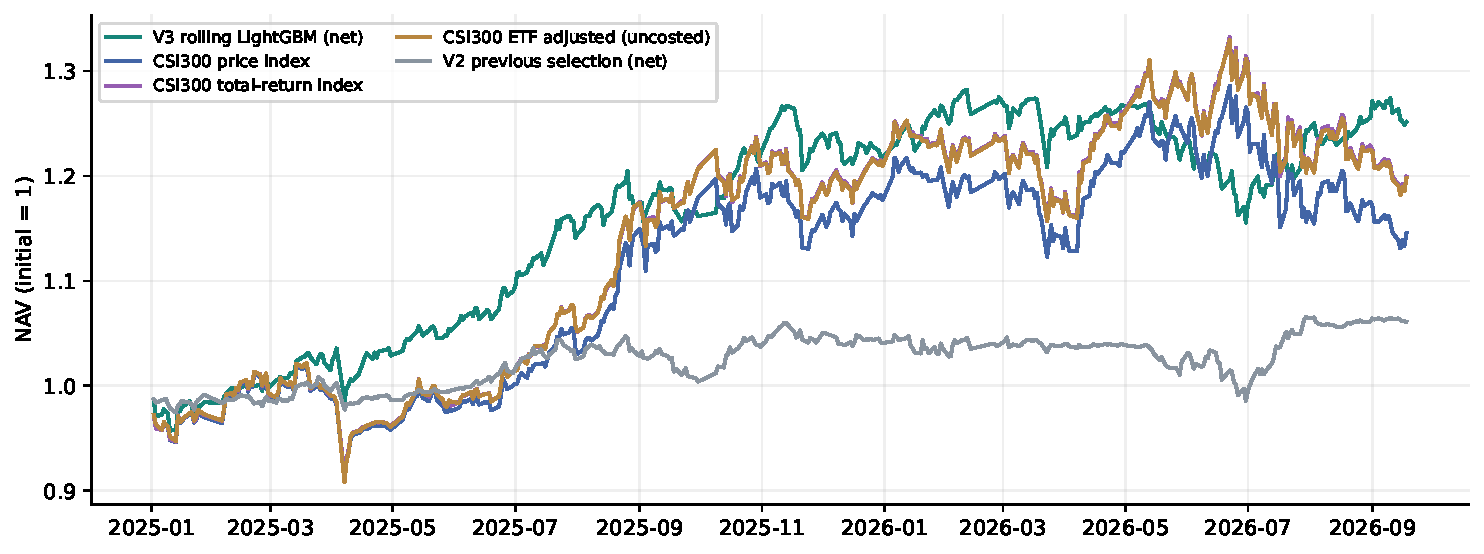
\includegraphics[width=.96\textwidth,height=.51\textheight,keepaspectratio]{figures/nav.pdf}\par
\scriptsize\begin{itemize}
\item 价格指数14.55\%，全收益指数19.94\%
\item 分别超过10.58和5.19个百分点
\end{itemize}
{\tiny PowerPoint每5日取点；完整417日曲线见报告与平台。}
\note{这张图使用二零二五年一月二日至二零二六年九月十八日相同的四百一十七个交易日。策略已经扣除实际费用，累计收益百分之二十五点一三，最大回撤百分之九点八八。沪深三百价格指数同期收益百分之十四点五五，计入红利再投资的全收益指数是百分之十九点九四。因此，策略分别超过十点五八和五点一九个百分点。这里不能把ETF代理改称全收益指数，也不能混淆百分点差和相对财富增长。为了避免首日亏损被抹掉，策略从期初资金起算，指数从前一交易日收盘起算。平台中的日期切片和策略比较采用完全相同的边界定义。}
\end{frame}

\begin{frame}{压力检查与落后年份}
\begin{block}{}提高费用后仍超过同期全收益指数\end{block}
\centering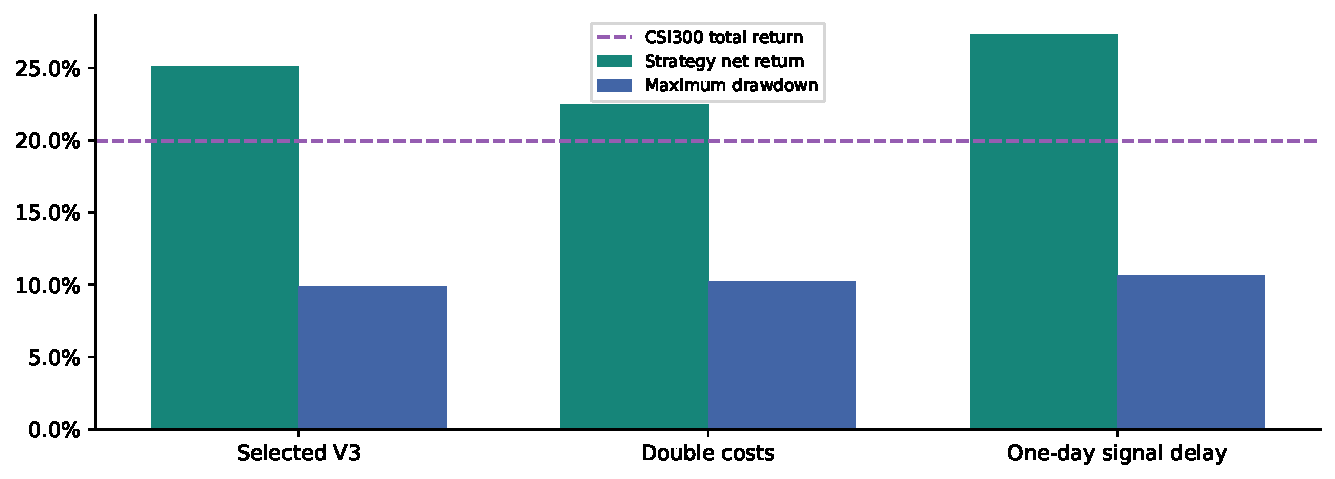
\includegraphics[width=.96\textwidth,height=.51\textheight,keepaspectratio]{figures/controls.pdf}\par
\scriptsize\begin{itemize}
\item 双倍费用：22.48\%；延迟一日：27.31\%
\item 2023起连续44.09\%，2024年落后价格指数
\end{itemize}
\note{收益结果还需要承受一些简单但实际的扰动。我们把买卖费用同时加倍，完整重跑账本，收益仍为百分之二十二点四八；把信号延迟一日，收益为百分之二十七点三一。延迟结果更好，不代表可以再把它挑成默认参数，否则压力测试又变成一次找冠军。另一个检查从二零二三年开始连续运行，不在每年年初重置资金，累计收益百分之四十四点零九，最大回撤百分之十九点七。但二零二四年仍然落后价格指数七点二八个百分点。这个年份提醒我们，长期累计领先不能被解释为每年都赢。接下来我们用平台工具把这种差异具体拆开。}
\end{frame}

\begin{frame}{工具一：同区间策略对比}
\begin{block}{}选择版本与日期，导出同一计算口径的结果\end{block}
\centering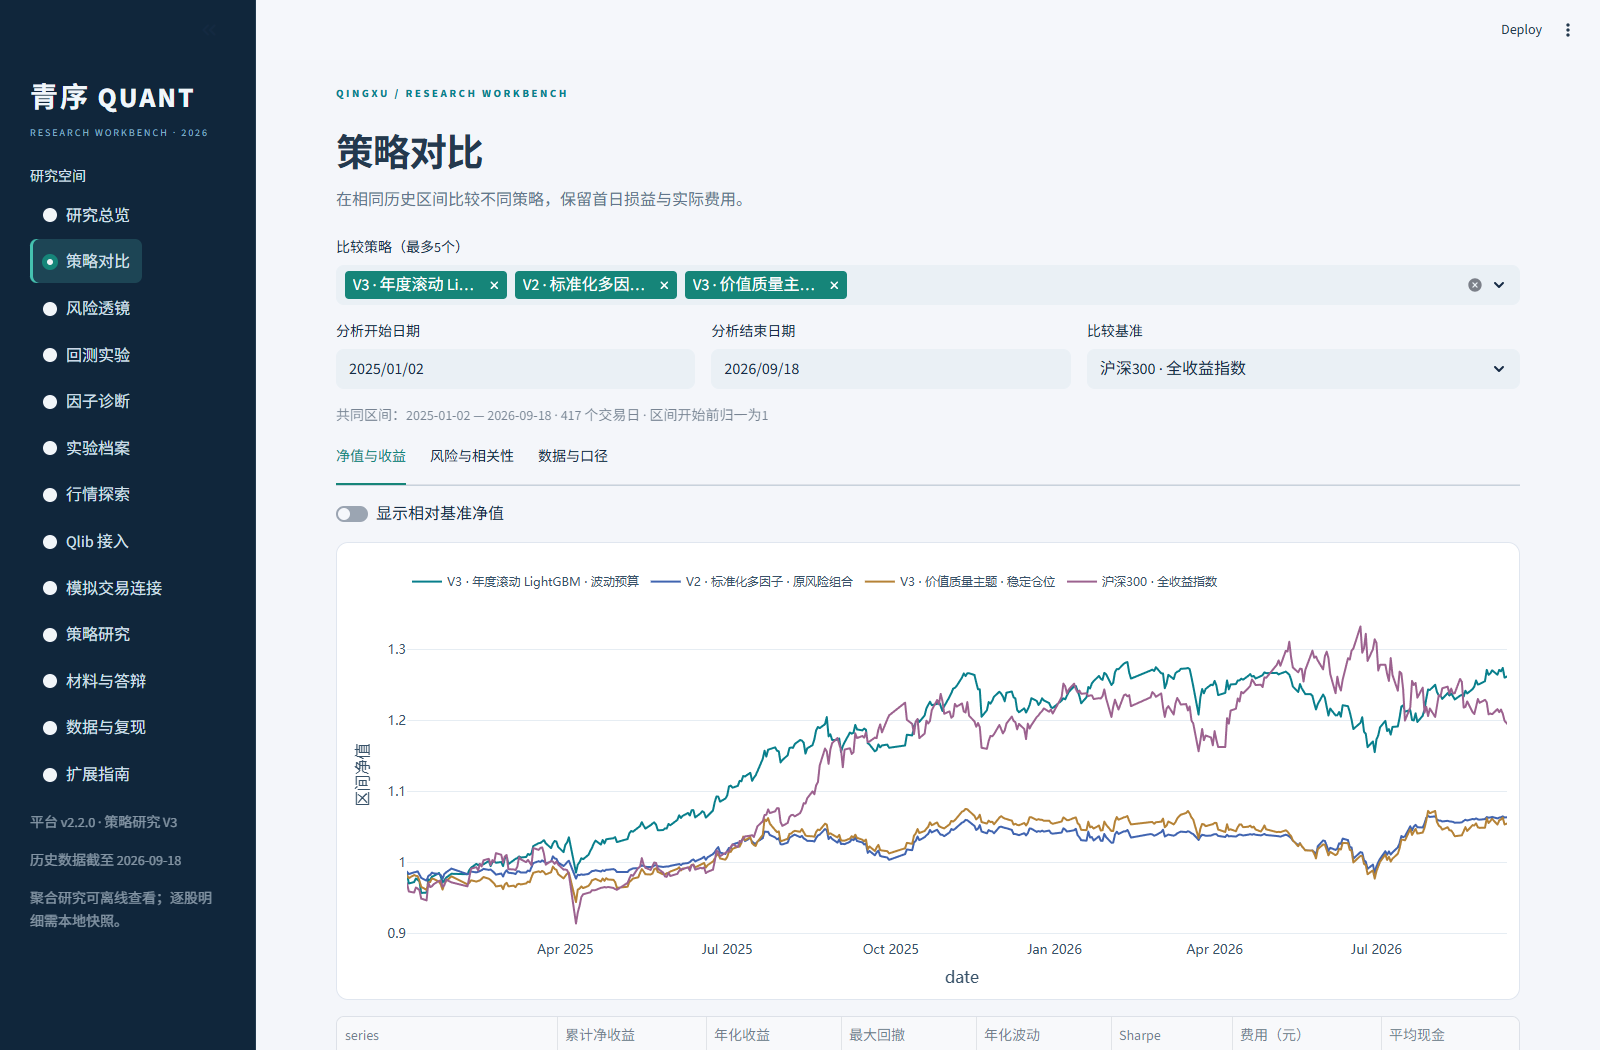
\includegraphics[width=.95\textwidth,height=.55\textheight,keepaspectratio]{figures/ui-v4-compare.png}\par
\scriptsize\begin{itemize}
\item 最多五版策略；价格或全收益基准
\item 累计/相对净值、回撤、相关性与指标表
\item 区间从前收盘起算，首日损益保留
\end{itemize}
\note{策略对比页解决的是公平比较问题。我们可以同时选择最多五个版本，限定相同日期，再选择价格指数或全收益指数。图表既可以看普通净值，也可以看策略净值除以基准净值后的相对表现。下面的表把收益、回撤、费用和现金比例放在一起，避免只比较一个收益数字。日期改变以后，系统使用所选首日前的净值作为起点，因此不会把首日损失归一掉。需要注意，这里是在切片一条已经运行的持仓路径，并不是从现金重新开仓；如果要改变实际交易参数，应该回到回测实验重新执行。所有图表、统计和计算假设可以一次下载为比较包，方便写报告或与组员核对。}
\end{frame}

\begin{frame}{工具二：风险透镜}
\begin{block}{}定位回撤、月份与现金配置的影响\end{block}
\centering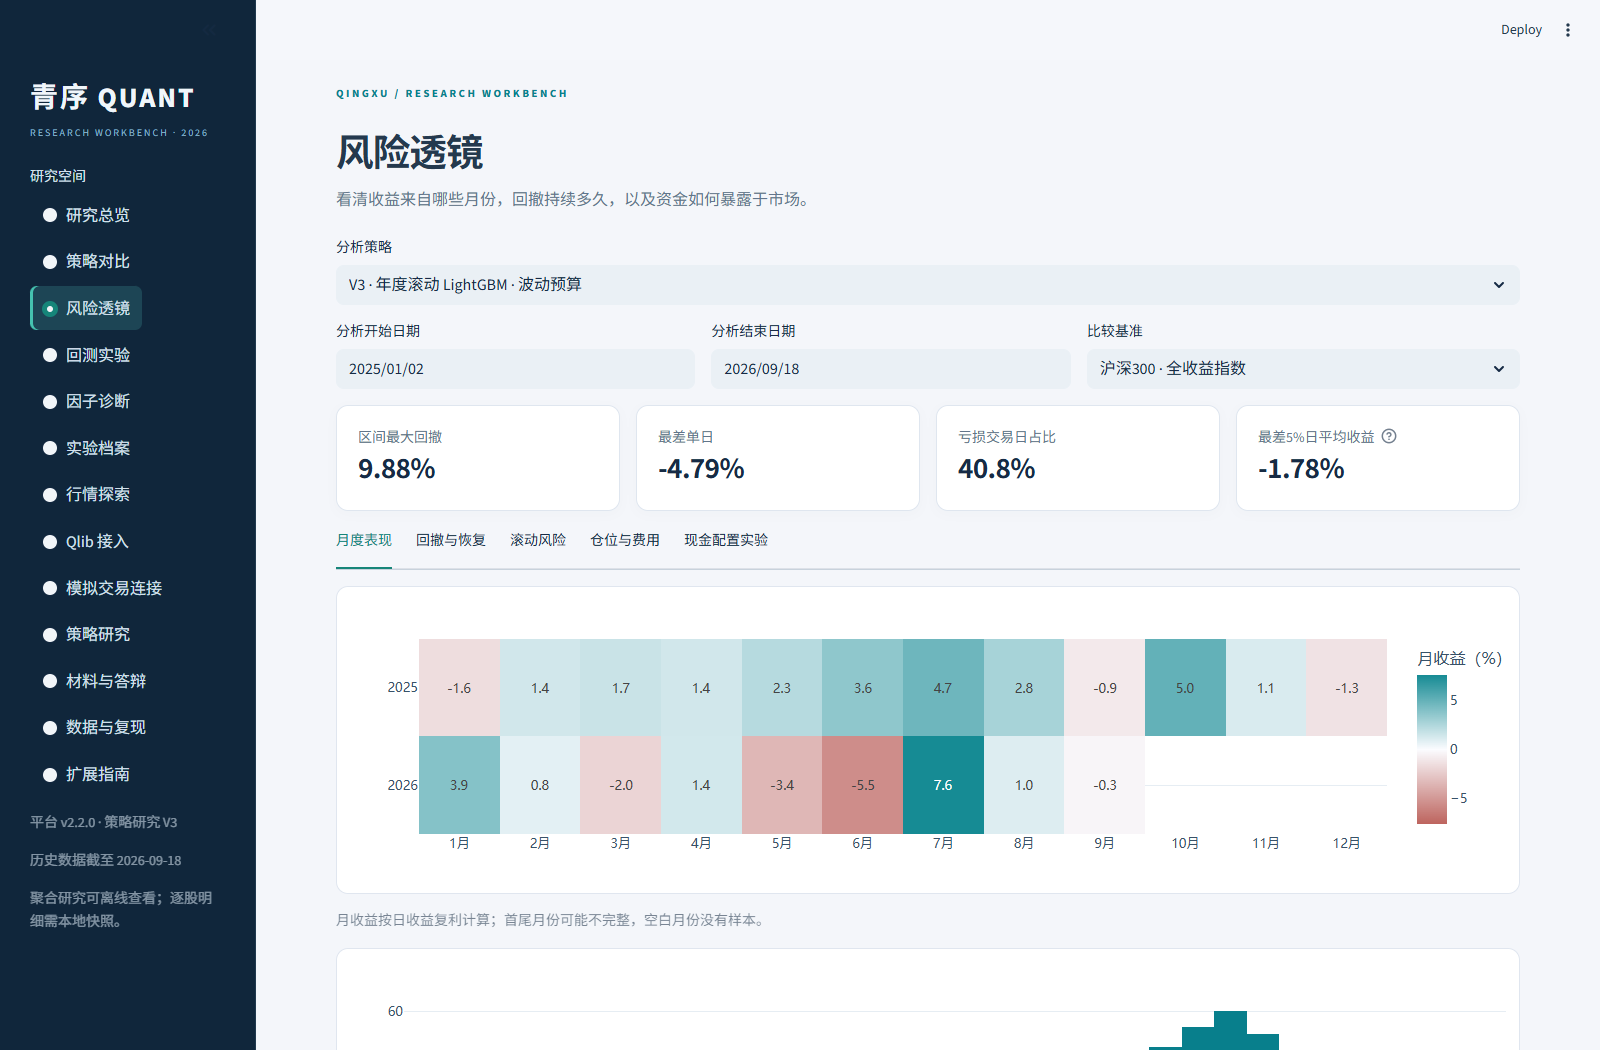
\includegraphics[width=.95\textwidth,height=.55\textheight,keepaspectratio]{figures/ui-v4-risk.png}\par
\scriptsize\begin{itemize}
\item 月收益日历、日收益分布、回撤恢复表
\item 60日滚动收益、波动与下行偏差
\item 现金/费用/换手；静态资金分配情景
\end{itemize}
\note{风险透镜把一个最大回撤数字拆成可以解释的过程。月收益日历能看出收益集中在哪些月份，回撤表则列出峰值、谷底、恢复日期和持续交易日。尚未恢复的回撤保留为空，不伪装成已经恢复。滚动曲线用最近六十个交易日计算收益与风险，不足窗口时不补值。现金和换手图让我们看到防御仓位以及费用发生在哪些时段。最后还有一个可以动手操作的现金配置实验：把部分初始资金投入策略，其余保持零利息现金，并输入通胀假设查看购买力。它是一种静态资金分配的算术情景，没有重新模拟资金规模对成交容量的影响，也不是新增的交易策略。}
\end{frame}

\begin{frame}{工具三：因子与行情探索}
\begin{block}{}把模型输入连接到具体日期和股票\end{block}
\small\begin{itemize}
\item 十二因子按日期诊断；行情按股票筛选
\item 因子卡、覆盖率、IC/Rank IC与分组诊断
\item 行情K线与成交量，真实数据缺失明确说明
\end{itemize}
\note{因子与行情入口可以把抽象模型拉回具体数据。我们可以先选择一个研究因子，阅读它的窗口、字段和方向，再查看形成日的样本覆盖、IC和分组结果。如果一个因子突然没有有效值，就能沿着日期检查价格、成交量或财报缺失，而不是直接把空值当成模型信号。行情页提供K线和成交量查询，方便检查异常价格和某次信号对应的市场背景。公开离线模式下，界面只展示已有的聚合证据；没有本机原始行情时不会伪造K线。这个入口也适合课堂提问，例如老师指定一只股票或一个日期，我们可以现场说明它的数据是否可见、因子是否有效，再讨论预测是否合理。}
\end{frame}

\begin{frame}{工具四：实验档案与研究笔记}
\begin{block}{}从一条净值曲线追到订单与配置\end{block}
\centering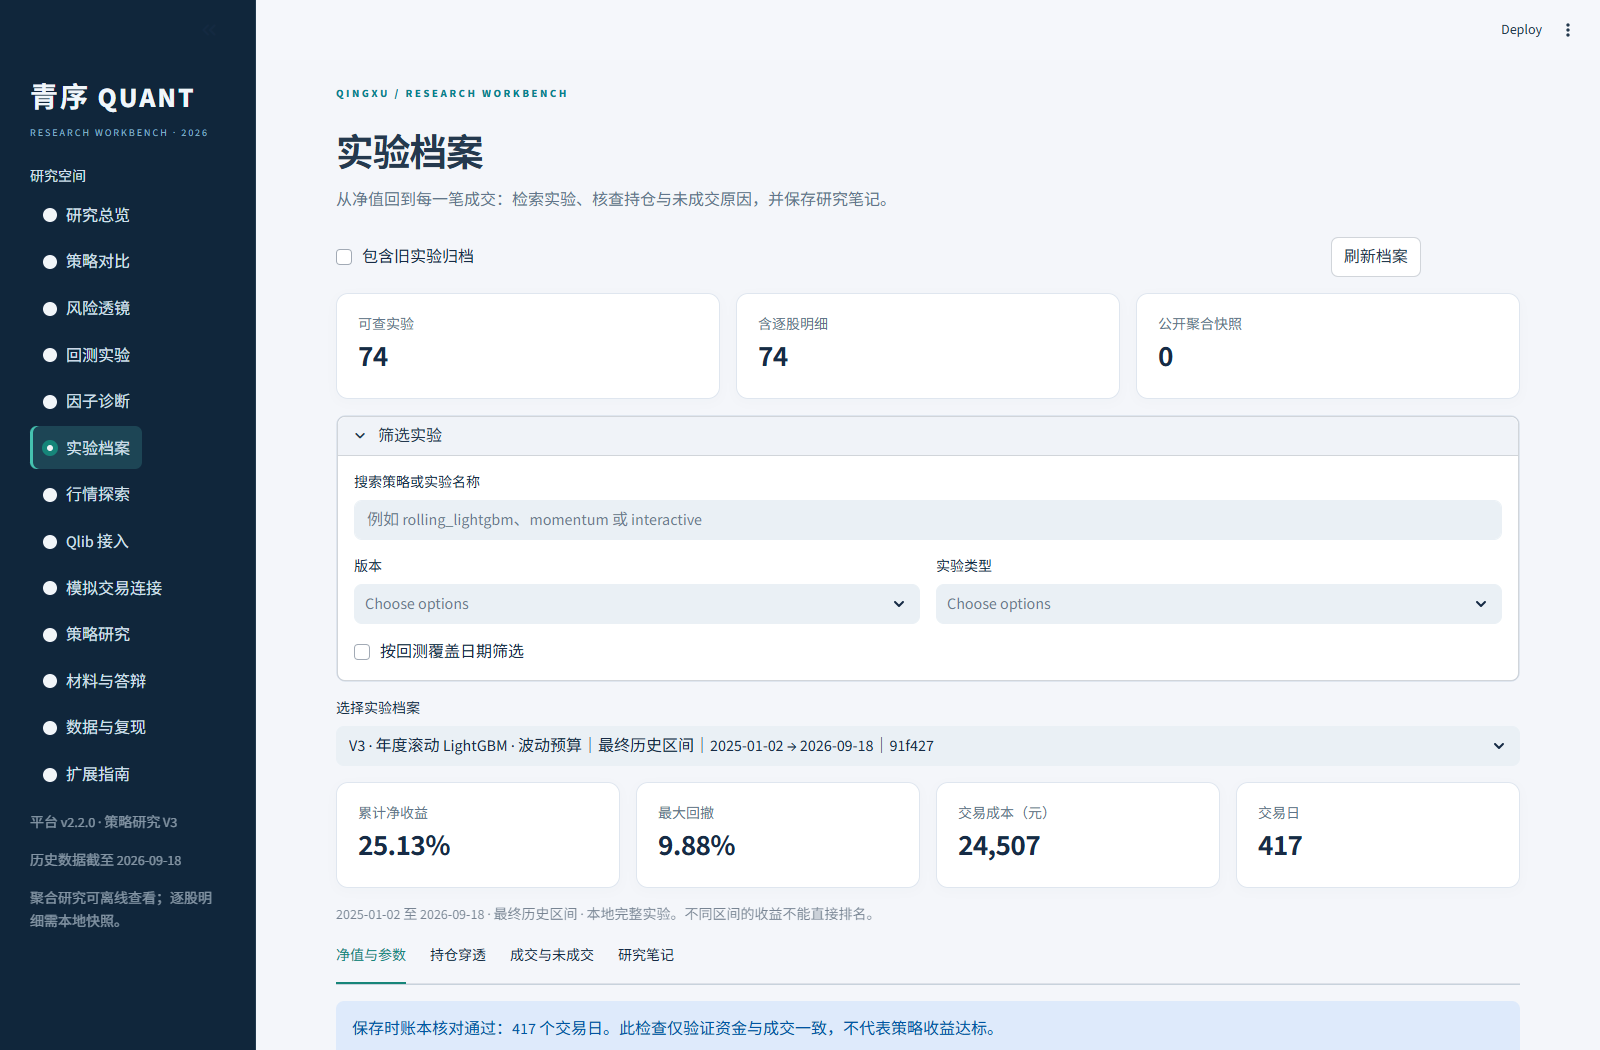
\includegraphics[width=.95\textwidth,height=.55\textheight,keepaspectratio]{figures/ui-v4-experiments.png}\par
\scriptsize\begin{itemize}
\item 按实验、日期、股票、成交状态检索
\item 查看资金、持仓、费用与来源身份
\item 保存本地笔记，导出研究记录
\end{itemize}
\note{实验档案让每次尝试都有可追溯的上下文。参数重跑会生成新的运行目录，档案页可以打开这次实验，检查实际使用的策略、日期、资金与费用。进一步按股票或订单状态筛选，就能解释一次涨停买不到、缺价估值或者部分成交对账本产生了什么影响。我们还加入本地研究笔记，用来记录这次改变了哪个假设、观察到什么现象、下一步需要验证什么。笔记与实验关联，但不改变历史账本。这样的设计比只保留最终冠军更有用，因为小组后续项目可以沿着旧实验继续工作。课堂演示时，我们会打开一个已完成实验并查看一笔订单，不让大家等待重新训练。}
\end{frame}

\begin{frame}{Qlib与外部工具连接}
\begin{block}{}Qlib原生8表达式与Alpha158配置已实测\end{block}
\begin{center}\small\begin{tabularx}{.97\textwidth}{lX}\toprule
接入层 & 实际结果与范围\\\midrule
Qlib数据桥 & 0.9.7 / 20股 / 33,754条日线\\
独立核验 & 8项表达式，269,554个数值核对\\
Alpha158 & 官方158项表达式实际执行\\
同花顺文件桥 & CSV导入与金额核对；账号/API未连接\\
\bottomrule\end{tabularx}\end{center}
\small\begin{itemize}
\item Qlib尚未训练新策略；V3历史结果保留
\item 同花顺尚未登录，未提交订单
\end{itemize}
\note{老师推荐Qlib，因此我们把它作为可复用的研究组件，而不是只在报告中放一个名字。Qlib 0.9.7在独立环境读取本地转换的数据；20股共33,754条日线，8个基础表达式与独立pandas计算逐项核对。共核对269,554个数值，有限值与缺失位置一致。另实际运行官方Alpha158的158项配置，158项至少有一个有限值，VWAP输入覆盖率100.0\%。这属于因子计算和数据接口验证，未训练Qlib交易策略，也未替换现有成交账本。一个外部因子接进来以后，仍然要经过我们自己的信息时点检查、诊断和同区间比较，不能因为来自知名库就直接上线。另一个连接是同花顺。同花顺/SuperMind文件桥已完成：可导出历史权重与代码、导入模拟成交CSV并校验金额、保存本地回执。账号/API未连接，未收到真实账户文件，未提交任何订单；现金流核对不等于盈利。课堂上应当清楚区分三种状态：能导出文件，能调用已授权的数据接口，以及能向交易系统提交订单。这三者不是同一件事。本项目的实证结果仍由本地研究账本产生。}
\end{frame}

\begin{frame}{现场演示顺序}
\begin{block}{}两分钟完成一次可复核的研究操作\end{block}
\small\begin{itemize}
\item 总览确认V3 → 对比V2与全收益指数
\item 风险透镜改日期 → 查看回撤恢复与月历
\item 因子或行情查询 → 实验档案检索订单
\item 下载比较包 → 保存一条研究笔记
\end{itemize}
\note{下面用约两分钟实际操作一次。先看研究总览，确认当前默认版本、数据区间和历史选择边界。进入策略对比，保留V3，再加入V2原预选，并将基准设为全收益指数，大家可以看到两版策略的差异。接着进入风险透镜，修改分析日期，指向月收益和最深回撤，说明这是一段持仓路径的切片。然后打开因子或行情页面，展示一个具体日期的样本。最后进入实验档案，筛选一笔订单，查看成交状态和费用，保存一条带有实验背景的笔记。如果教室网络或现场页面不稳定，我们切换到预先保存的真实截图继续说明；演示不现场下载数据，也不现场等待模型重训。}
\end{frame}

\begin{frame}{验证与复现}
\begin{block}{}公开聚合证据可离线检查，真实重跑要求本机数据\end{block}
\small\begin{itemize}
\item 21组V3研究/压力账本，独立环境复算
\item 主环境102通过、1跳过；Qlib隔离5通过
\item 公开数据分析与私有原始数据重跑分层
\item Git版本、配置、SHA与导出包共同定位结果
\end{itemize}
\note{我们用两类检查支持这些功能。第一类验证研究核心，包括订单、费用、现金、持仓和净值的独立重建，第三版共有二十一组研究与压力账本，并在独立环境中复算。第二类验证新增工具容易出错的边界，例如首日损失是否保留，不同策略是否比较相同日期，缺失日是否被偷偷插值，以及未恢复回撤是否被误记成恢复。公开仓库提供真实聚合日账本，所以没有账号也能打开对比与风险页。真正重新训练或者查看逐股行情，则需要本机合法取得的数据。我们提供源码、固定依赖、操作说明和版本号，让下一位同学能够判断自己是在复现哪一个结果。}
\end{frame}

\begin{frame}{结论与下一步}
\begin{block}{}保留有效工具，也保留尚未解决的问题\end{block}
\small\begin{itemize}
\item 平台：可比较、可解释、可追踪、可扩展
\item 策略：该历史区间扣费后超过两类沪深300基准
\item 限制：历史重选、固定池与执行近似
\item 下一步：冻结规则，积累真正的新数据验证
\end{itemize}
\note{最后回到本项目的目标。我们交付的不只是一个收益数字，而是能够继续研究的平台：可以输入新信号，按统一规则回测，公平比较版本，解释风险，再把证据留给下一次实验。当前策略在这段历史上超过价格指数和全收益指数，但我们没有删除原始亏损、预选失败和落后年份。它仍然存在固定股票池、厂商历史修订以及成交近似的限制，历史重选也意味着还不能宣称独立盲测成功。下一步最有价值的工作是冻结当前规则，持续积累未见过的新数据，然后按相同标准检查。以上就是我们的展示，谢谢各位老师和同学，欢迎针对因子、账本和平台操作提问。}
\end{frame}

\begin{frame}{备份：统计口径}
\begin{block}{}初始资金参与首日收益与最大回撤\end{block}
\[r_t=\frac{NAV_t}{NAV_{t-1}}-1,\qquad DD_t=1-\frac{NAV_t}{\max_{0\leq s\leq t}NAV_s}\]
\small\begin{itemize}
\item 收益：NAV终值 / 区间前收盘 − 1
\item 回撤：1 − NAV / 包含初始值的历史高点
\item 下行偏差：全部观察日作分母，目标为零
\item 月度收益复利；重叠20日标签不能连乘为净值
\end{itemize}
\note{如果老师追问统计公式，可以用这一页说明。区间第一天收益不是零，而是第一天收盘净值与前一日净值或初始资金的比值。最大回撤的高水位也包含初始资金，因此一开始就亏损不会被遗漏。年化波动采用样本标准差乘根号二百五十二，下行偏差把正收益日记为零，但分母仍然是全部观察日。月度收益由日收益复利得到，首尾不足一个月会明确显示。因子二十日远期标签存在重叠，它适合诊断排序关系，不能直接连乘当作真实投资净值。}
\end{frame}

\begin{frame}{备份：答辩问题}
\begin{block}{}如实解释模型选择、现金与连接状态\end{block}
\small\begin{itemize}
\item 为什么不用CNN？因子列没有天然局部邻接
\item 为什么不是最高收益版本？验证回撤门槛
\item 现金情景能当策略吗？只是静态资金分配
\item Qlib接入范围：因子计算，尚未训练新策略
\end{itemize}
\note{如果问为什么没有按最初建议使用CNN，我们的回答是，表格因子列没有天然空间邻接，先用线性模型、受限树模型和小型MLP比较更合理。如果问为什么没有选收益最高的稳定树模型，是因为它的验证回撤超过了事先保留的风险门槛。如果问现金实验是否就是一个新策略，需要说明它只是资金缩放情景，改变交易规模仍然需要重新回测。最后，Qlib数据表达式接入、同花顺文件桥和真正的交易授权必须分别回答，以最终运行证据为准，不能把准备好的接口说成已经接通的交易账户。}
\end{frame}
\end{document}